\documentclass[12pt,a4paper,openright,twoside]{book}
\usepackage[italian]{babel}
\usepackage[utf8]{inputenc}
\usepackage{fancyhdr}
\usepackage{indentfirst}
\usepackage{graphicx}

\pagestyle{fancy}

\oddsidemargin=30pt
\evensidemargin=20pt

% Sillabazione
\hyphenation{}

% Intestazione e piè di pagina
\pagestyle{fancy}\addtolength{\headwidth}{20pt}
\renewcommand{\chaptermark}[1]{\markboth{\thechapter.\ #1}{}}
\renewcommand{\sectionmark}[1]{\markright{\thesection \ #1}{}}
\rhead[\fancyplain{}{\bfseries\leftmark}]{\fancyplain{}{\bfseries\thepage}}
\cfoot{}

% Interlinea
\linespread{1.3}

\begin{document}

%
% Dedica
%
\begin{titlepage}
  % No numero di pagina
  \thispagestyle{empty}
  \topmargin=6.5cm
  \raggedleft
  \large
  \em A Chiara
\end{titlepage}

\pagenumbering{roman}

\chapter*{Introduzione}
\rhead[\fancyplain{}{\bfseries
INTRODUZIONE}]{\fancyplain{}{\bfseries\thepage}}
\lhead[\fancyplain{}{\bfseries\thepage}]{\fancyplain{}{\bfseries
INTRODUZIONE}}
\addcontentsline{toc}{chapter}{Introduzione}

``Comunicare, sempre'' è un imperativo sempre più assordante. In
quest'ottica, negli ultimi anni, si è diffusa rapidamente la
comunicazione vocale su sistemi VoIP, comunemente nota come
``telefonia via Internet''. Questa tecnologia permette conversazioni
audio/video tra due o più partecipanti senza limiti di distanza e di
tempo, al prezzo di una normale connessione Internet a banda larga e
di un computer.

Contemporaneamente e indipendentemente si sono affermate le reti senza
fili su protocollo 802.11, le reti wireless. L'uso combinato delle due
tecnologie permetterebbe una comunicazione audio-video economica, su
scala mondiale e non limitata negli spostamenti dei
partecipanti. Esistono però due limitazioni castranti per questo tipo
di applicazione: lo scarso raggio di copertura degli apparecchi
wireless e l'eterogeneità delle reti senza fili. I dispositivi WiFi,
limitati a un raggio d'azione tipicamente circoscritto alla pianta di
un edificio, escono duramente sconfitti dal confronto con la capacità
dei tradizionali cellulari di restare costantemente connessi alla rete
telefonica nazionale e internazionale durante ogni tipo di
spostamento. Tecnicamente l'accesso a una rete WiFi viene fornito da
un dispositivo chiamato \emph{access point}, che permette ai vari
dispositivi 802.11 di collegarsi via radio. Il raggio del segnale
molto ridotto, entro i 300 metri, e una suscettibilità molto alta alle
interferenze e agli ostacoli fisici intralciano la mobilità. Supplire
alla scarsa portata passando di rete in rete durante gli spostamenti
non è comunque facile, perché ogni rete senza fili è un mondo a sè; a
differenza di un cellulare, che può via via associarsi a diversi
ripetitori rimanendo sempre identificato dallo stesso numero di
telefono, le interfacce WiFi cambiano indirizzo IP, e quindi identità,
ogni volta che si associano con un access point di una rete
differente, rendendo impossibile la comunicazione continua, costante e
senza interruzioni necessaria per una conversazione telefonica.

Il progetto Robust Wireless Medium Access punta a risolvere questi due
problemi con un approccio \emph{cross layer}: l'alta percentuale
d'errore nel collegamento senza fili viene mitigata da un meccanismo
di rilevazione d'errore e ritrasmissione installato nel dispositivo
dell'utente; l'impossibilità di cambiare rete WiFi senza interruzioni
viene risolta utilizzando più interfacce di rete per dispositivo e
utilizzando un Proxy Server che gestisca in modo trasparente i
cambiamenti di indirizzo IP nelle interfacce del client.

Il meccanismo di \emph{error recovery} e \emph{load balancing} può
applicare diversi algoritmi, che devono essere analizzati e
confrontati per individuare il più adatto. La struttura del progetto
rende molto difficile, se non praticamente impossibile, condurre delle
prove nella realtà; per questo si è scelto di eseguire dei test in una
simulazione.

In questo documento (TODO: tesi, lavoro, opera?) descriverò
inizialmente il funzionamento del meccanismo RWMA, per poi presentare
il progetto e l'implementazione di un simulatore a eventi discreti che
possa modellare i vari componenti di rete con i rispettivi algoritmi
di QoS.

TODO: nel primo capitolo

TODO: nel secondo capitolo

TODO: etc.

% Indice
\tableofcontents
\rhead[\fancyplain{}{\bfseries\leftmark}]{\fancyplain{}{\bfseries\thepage}}
\lhead[\fancyplain{}{\bfseries\thepage}]{\fancyplain{}{\bfseries
INDICE}}

% Capitoli
\chapter{Scenario}
\lhead[\fancyplain{}{\bfseries\thepage}]{\fancyplain{}{\bfseries\rightmark}}
\pagenumbering{arabic}

Lo scenario da considerare è illustrato in figura \ref{fig:scenario} e
originariamente presentato nell'articolo di ricerca ``Robust Wireless
Medium Access for VoWLAN Applications: A Cross--Layer QoS Mechanism''
\cite{bib:rwma}. Si assuma che esista una comunicazione vocale tra due
sistemi A e B, in figura rappresentati come ``Alice'' e ``Bob''. Il
sistema A è un dispositivo mobile dotato di più di un'interfaccia
wireless, ognuna delle quali è associata con un diverso access
point. I vari access point possono appartenere a infrastrutture di
rete e domini differenti e quindi essere completamente indipendenti
l'uno dall'altro. Gli access point sono connessi a Internet attraverso
una connessione via cavo. Il sistema B è un dispositivo fisso,
connesso a Internet via cavo attraverso una comune allacciamento
Internet a banda larga, come ADSL o fibra ottica.

\begin{figure}[t]
\centering
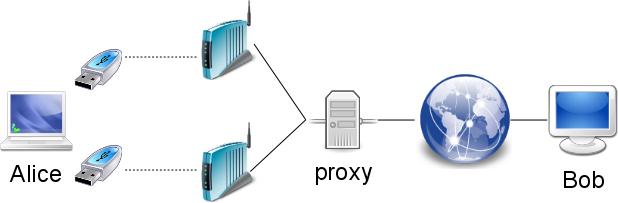
\includegraphics[width=\textwidth]{img/scenario}
\caption{Scenario}
\label{fig:scenario}
\end{figure}

La comunicazione VoIP tra i sistemi A e B si affida quindi a due tipi
di connessione: quella wireless, tra A e gli access point, e quella
via cavo tra gli access point e B.

\section{Vincoli qualitativi}

Come mostrato, il percorso dei dati da un sistema VoIP all'altro deve
attraversare segmenti camblati e altri senza fili; di questi gli
ultimi sono i più problematici, perchè soffrono di tre gravi
inconvenienti: alta latenza, frequenti errori di trasmissione e
interruzione e ripristino della connessione nel cambiare access
point. Latenza ed errori frequenti possono degradare la qualità di una
comunicazione VoIP via wireless fino a renderla inintelleggibile,
mentre l'interruzione della connessione durante il passaggio da un
access point a un altro impedisce la mobilità del sistema obbligando
l'utente a restare nei pressi del ripetitore wireless in uso, pena la
disconnessione e l'interruzione della comunicazione.

Per garantire una buona qualità del servizio, il sistema RWMA deve
operare soddisfando vincoli di interattività, affidabilità e mobilità.

\subsection{Interattività}
L'interattività di una conversazione VoIP è influenzata dalla latenza
dei pacchetti che ne compongono il flusso di rete. La latenza di
trasmissione è definita come il tempo trascorso dall'istante del
campionamento della voce sul sistema di origine all'instante di
riproduzione audio della stessa voce sul sistema di destinazione. Le
raccomandazioni ITU--T \cite{itu-t} indicano 150 ms come latenza
massima di una comunicazione VoIP soddisfacente; al di sopra di questa
soglia l'interattività della conversazione non è più accettabile.

\subsection{Affidabilità}
L'affidabilità di una conversazione VoIP dipende dalla capacità della
rete di portare a destinazione quanti più pacchetti possibili. Un
pacchetto è considerato perso quanto viene trasmesso dal sistema
origine e non viene ricevuto dal sistema destinazione. Per condurre
una conversazione comprensibile è necessario che la percentuale di
pacchetti persi resti al di sotto del 10\% \cite{itu-t}.

\subsection{Mobilità}
La mobilità dell'utente è fortemente limitata dallo scarso raggio
d'azione offerto dalle attuali apparecchiature WiFi. Le interfacce
WiFi sono in grado di interrompere l'associazione con l'access point
in uso per crearne una nuova con un secondo solo quando i suddetti
access point sono parte della stessa infrastruttura di rete. Questa
limitazione deriva direttamente dal funzionamento del protocollo IP:
cambiando rete di accesso l'interfaccia wireless riceve un nuovo
indirizzo IP e deve reinstaurare la connessione da zero. Ciò che si
vuole è invece un processo di disconnessione e riconnessione
trasparente all'applicazione, in modo che la chiamata VoIP non venga
interrotta, e rapido, in modo da non violare il requisito di
interattività precedentemente esposto.

\section{Il meccanismo RWMA}
Il meccanismo RWMA, schematizzato in figura \ref{fig:rwma} mira a
risolvere i tre problemi di interattività, affidabilità e mobilità
utilizzando un approccio TODO CONTINUA QUI

\begin{itemize}
\item TED (Transmission Error Detection)
\item ULB (UDP Load Balancer)
\item IM (Interface Monitor)
\item PS (Proxy Server)
\end{itemize}

TODO

\begin{verbatim}
           +-----------------+                   +-------+
SOFTPHONE  |          iface0 +----AP0------------+       |
 |         |                 |                   |       |
 |         |          iface1 +----AP1------------+       |
 +---lo----+ LOAD            |        INTERNET   | PROXY +-...
           | BALANCER   ...  | ................. |       |
 +-MSG_ERR-+                 |                   |       |
 |         |          ifacen +----APn------------+       |
KERNEL     +-------------+---+                   +-------+
                         |
                    INTERFACE
                     MANAGER
\end{verbatim}

\chapter{Dettagli tecnici}


\chapter{Simulazione}
% Obiettivi a cui punto. Spiegazione soluzioni, algoritmi e scelte
% effettuate.
ULB e Proxy Server sono i componenti del sistema che eseguono le
scelte necessarie a garantire una migliore qualità del
servizio. Mentre i componenti Interface Manager, Linux Kernel,
Softphone, Wireless Interface e Access Point hanno comportamenti
predefiniti e sostanzialmente non modificabili, ULB e PS possono
implementare diverse tecniche di analisi della qualità delle
connessioni e varie strategie di recupero degli errori.

Compito del simulatore è fornire un ambiente virtuale in cui questi
diversi algoritmi possano essere eseguiti, analizzati e confrontati.

È importante notare che, a questo stadio di sviluppo, il simulatore
non punta al realismo della simulazione. Per esempio, lo scenario
wireless è di molto semplificato, non venendo presi in considerazione
parametri fisici come la qualità del segnale radio in relazione alla
distanza di un client dall'access point. Tutti i dettagli di un link
wireless sono astratti dietro ai parametri di banda, latenza e
probabilità di errore; in particolare la rilevazione dell'ultimo
parametro sarà fondamentale per determinare la scelta dell'interfaccia
migliore. In quest'ottica, per simulare un calo di qualità del segnale
wireless dovuto all'aumentare della distanza tra client e access point
è sufficiente decidere quanto questo evento incida sulla probabilità
d'errore del collegamento e modificarla di conseguenza.

\section{Obiettivi simulatore}
Il simulatore è stato progettato secondo i principi di
\begin{itemize}
\item modularità
\item componibilità
\item generalità
\end{itemize}

\subsection{Modularità}
Modularità significa che i simulatori possono essere combinati tra di
loro per rappresentare nuovi scenari con componenti esistenti; per
esempio un'oggetto simulante un'interfaccia wireless in modo
soddisfacente, è autonomo e riutilizzabile in ogni scenario che
necessiti di un'interfaccia wireless. Questo permette il riuso del
codice in modo estremamente diretto.

\subsection{Componibilità}
Componibilità significa che ogni simulatore che partecipa in una
simulazione può essere a sua volta composto da più simulatori che
costituiscono le sue parti interne; questo permette di mantenere
gestibile la complessità della simulazione, senza dover sacrificare il
livello di dettaglio voluto.

\subsection{Generalità}
Il simulatore vuole essere un framework il più possibile
generale. L'obiettivo è essere utilizzabile in qualsiasi contesto in
cui il problema sia definibile in termini di eventi discreti.


\section{Obiettivi simulazione}
Confrontare i risultati:
\begin{itemize}
\item stesso scenario, algoritmi ULB differenti
\item stesso scenario, stesso algoritmo, parametri algoritmo differenti
\item scenari diversi per lo stesso algoritmo
\end{itemize}
Da tutto questo tirare fuori l'algoritmo migliore.

\section{Problemi}
Questa sezione illustra i problemi che devono essere affrontati dagli
algoritmi implementati nell'ULB. La sezione successiva mostrerà alcune
soluzioni e le confronterà tra loro.

\subsection{Ritrasmissione in tempi brevi}
ULB deve attendere le notifiche del TED e ritrasmettere i datagram che
sono stati segnalati come persi, ma senza superare i 150ms di ritardo.

\subsection{Valutazione interfacce}
ULB deve monitorare il comportamento delle varie interfacce dell'host
su cui viene eseguito e valutarne la qualità. L'interfaccia che
risulta essere la migliore viene utilizzata per l'invio dei dati. È
necessario definire sia quali siano i parametri secondo cui valutare
la qualità di un'interfaccia, sia le strategie di monitoraggio e
misurazione di questi parametri. La valutazione comprende sia
l'attività \emph{first hop} tra interfaccia e access point, sia quella
\emph{full path} tra interfaccia e Proxy Server.

\subsection{Rilevazione delle capacità del firmware}
I firmware delle schede di rete wireless sono in grado di notificare
sia l'avvenuta trasmissione di un datagram (ACK), sia la mancata
trasmissione (NAK). Putroppo non esiste uniformità di comportamento
tra i vari modelli sul mercato, ed è possibile che il firmware di una
scheda sia in grado di notificare solo ACK, oppure solo NAK, oppure
entrambi. Mancando un meccanismo nel kernel Linux per conoscere con
certezza le capacità di ogni firmware, ULB deve dedurle dal
comportamento osservato.

\subsubsection{Il problema del firmware silenzioso}
Il tipo di firmware si deduce dal tipo di notifiche ricevute dallo
stesso ed è quindi un meccanismo banale. Esistono però due casi in cui
il firmware può rimanere ``silenzioso'' e quindi impossibile da
rilevare:
\begin{enumerate}
\item quando una connessione pessima, che perde tutti i pacchetti,
  viene gestita da un firmware ACK che notifica solo successi, oppure
\item quando una connessione ottima, che non perde nessun pacchetto,
  viene gestita da un firmware NAK che notifica solo fallimenti.
\end{enumerate}
Non esiste un comportamento predefinito che soddisfi entrambe le
situazioni: la strategia del ritrasmettere ogni datagram che non
riceva notifiche entro un certo timeout funziona solo nella prima
situazione e risulta completamente inadeguato nella seconda.

\subsection{Conversazione unidirezionale}
Poichè l'host su cui risiede il softphone è dotato di più interfacce,
il Proxy Server si trova nella necessità di scegliere a quale tra
queste debba inviare i dati. Normalmente la scelta cade
sull'interfaccia che ha spedito gli ultimi dati ricevuti: se ULB l'ha
scelta come interfaccia migliore, il Proxy Server può fidarsi. Può
però accadere che il softphone non invii alcun dato perchè l'utente si
limita ad ascoltare; in questo caso il Proxy Server non ha cognizione
di quale sia l'interfaccia a cui inviare i dati.

\section{Soluzioni}
Tutti gli algoritmi sono stati progettati in modo da essere il più
possibile economici in termini di banda, tempi e energia.

Economia di banda significa limitare al minimo indispensabile
l'overhead nelle trasmissioni. In un contesto \emph{multi-homed} dove
ogni host possiede mediamente dalle due alle quattro interfacce,
ognuna di queste genera il proprio overhead che si va a sommare a
quello generato dalle altre.

L'economia di tempi è richiesta dalla caratterizzazione \emph{soft
  real-time} del problema, per cui un risultato ottenuto in ritardo
diventa inutilizzabile o fuorviante.

L'economia di energia dipende dalla natura dei client, che sono
tipicamente dispositivi mobili alimentati a batteria. Le interfacce
wireless sono periferiche avide di consumi e moltiplicandone il numero
si rischia di abbattere l'autonomia del client. Ancora una volta,
limitare l'overhead è l'unica via.

\subsection{Ritrasmissione in tempi brevi}
Fissato il ritardo massimo a 150ms, ULB associa un timeout di tale
durata ad ogni datagram ricevuto dal softphone. Scaduto il timeout il
datagram viene scartato.

\subsection{Valutazione interfacce}
Si è scelto di suddividere la valutazione di ogni interfaccia WiFi in
due sottovalutazioni differenti: una che considera il comportamento
nel \emph{first hop} e un'altra che considera quello nel \emph{full
  path}.

\subsubsection{First hop}
La valutazione \emph{first hop} rappresenta la qualità del
collegamento wireless tra interfaccia e access point, ed è una
funzione delle notifiche TED.
% TODO formula.

\subsubsection{Full path}
La valutazione \emph{full path} rappresenta l'affidabilità di tutto il
percorso dall'interfaccia al proxy server e ritorno. Ogni interfaccia
spedisce ogni 500ms un datagram che viene rispedito indietro dal Proxy
Server, come un semplice ping.

\chapter{Simulatore}
Implementazione del simulatore.

\chapter{Valutazioni}
Metriche con cui valuto il mio sistema. Deduzioni su misurazioni
effettuate. Perchè ho misurato certe cose e non altre.

\chapter*{Conclusioni}
\rhead[\fancyplain{}{\bfseries
CONCLUSIONI}]{\fancyplain{}{\bfseries\thepage}}
\lhead[\fancyplain{}{\bfseries\thepage}]{\fancyplain{}{\bfseries
CONCLUSIONI}}
\addcontentsline{toc}{chapter}{Conclusioni}
Un temerario che scriva una patch per ns2.

\renewcommand{\chaptermark}[1]{\markright{\thechapter \ #1}{}}
\lhead[\fancyplain{}{\bfseries\thepage}]{\fancyplain{}{\bfseries\rightmark}}
\appendix
\chapter{Codice de-sim}
\rhead[\fancyplain{}{\bfseries Appendice \thechapter: Codice de-sim}]{\fancyplain{}{\bfseries\thepage}}
prova

\chapter{Codice ulb-sim}
\rhead[\fancyplain{}{\bfseries Appendice \thechapter: Codice ulb-sim}]{\fancyplain{}{\bfseries\thepage}}
prova

\begin{thebibliography}{90}
\rhead[\fancyplain{}{\bfseries \leftmark}]{\fancyplain{}{\bfseries
\thepage}}
\addcontentsline{toc}{chapter}{Bibliografia}
\bibitem{bib:rwma} V. Ghini, G. Lodi, F. Panzieri, ``Robust Wireless
  Medium Access for VoWLAN Applications: A Cross--Layer QoS
  Mechanism'', Maggio 2008
\bibitem{itu-t} ITU--T Recommendation G. 114, ``One--way Transmission
  Time'', May 2003
\bibitem{al} V. Ghini, G. Lodi, F. Panzieri, ``Always Best Packet
  Switching: the Mobile VoIP Case Study'', Achademy Plublisher,
  Journal of Communications, accepted for publication.
\end{thebibliography}

\clearpage{\pagestyle{empty}\cleardoublepage}
\chapter*{Ringraziamenti}
\thispagestyle{empty}
Grazie, grazie al cazzo.
\end{document}
